\section{Versuchsaufbau/-durchführung}
\textbf{autocomplete python wieder installieren}
Ein zu untersuchender Würfel, dessen Hülle aus Aluminium besteht, beinhaltet neun kleinere Würfel der Länge $l$,
die jeweils aus Aluminium oder Blei gefertigt sind (vgl. \ref{fig: aufbau}).

\begin{figure}[h]
  \centering
  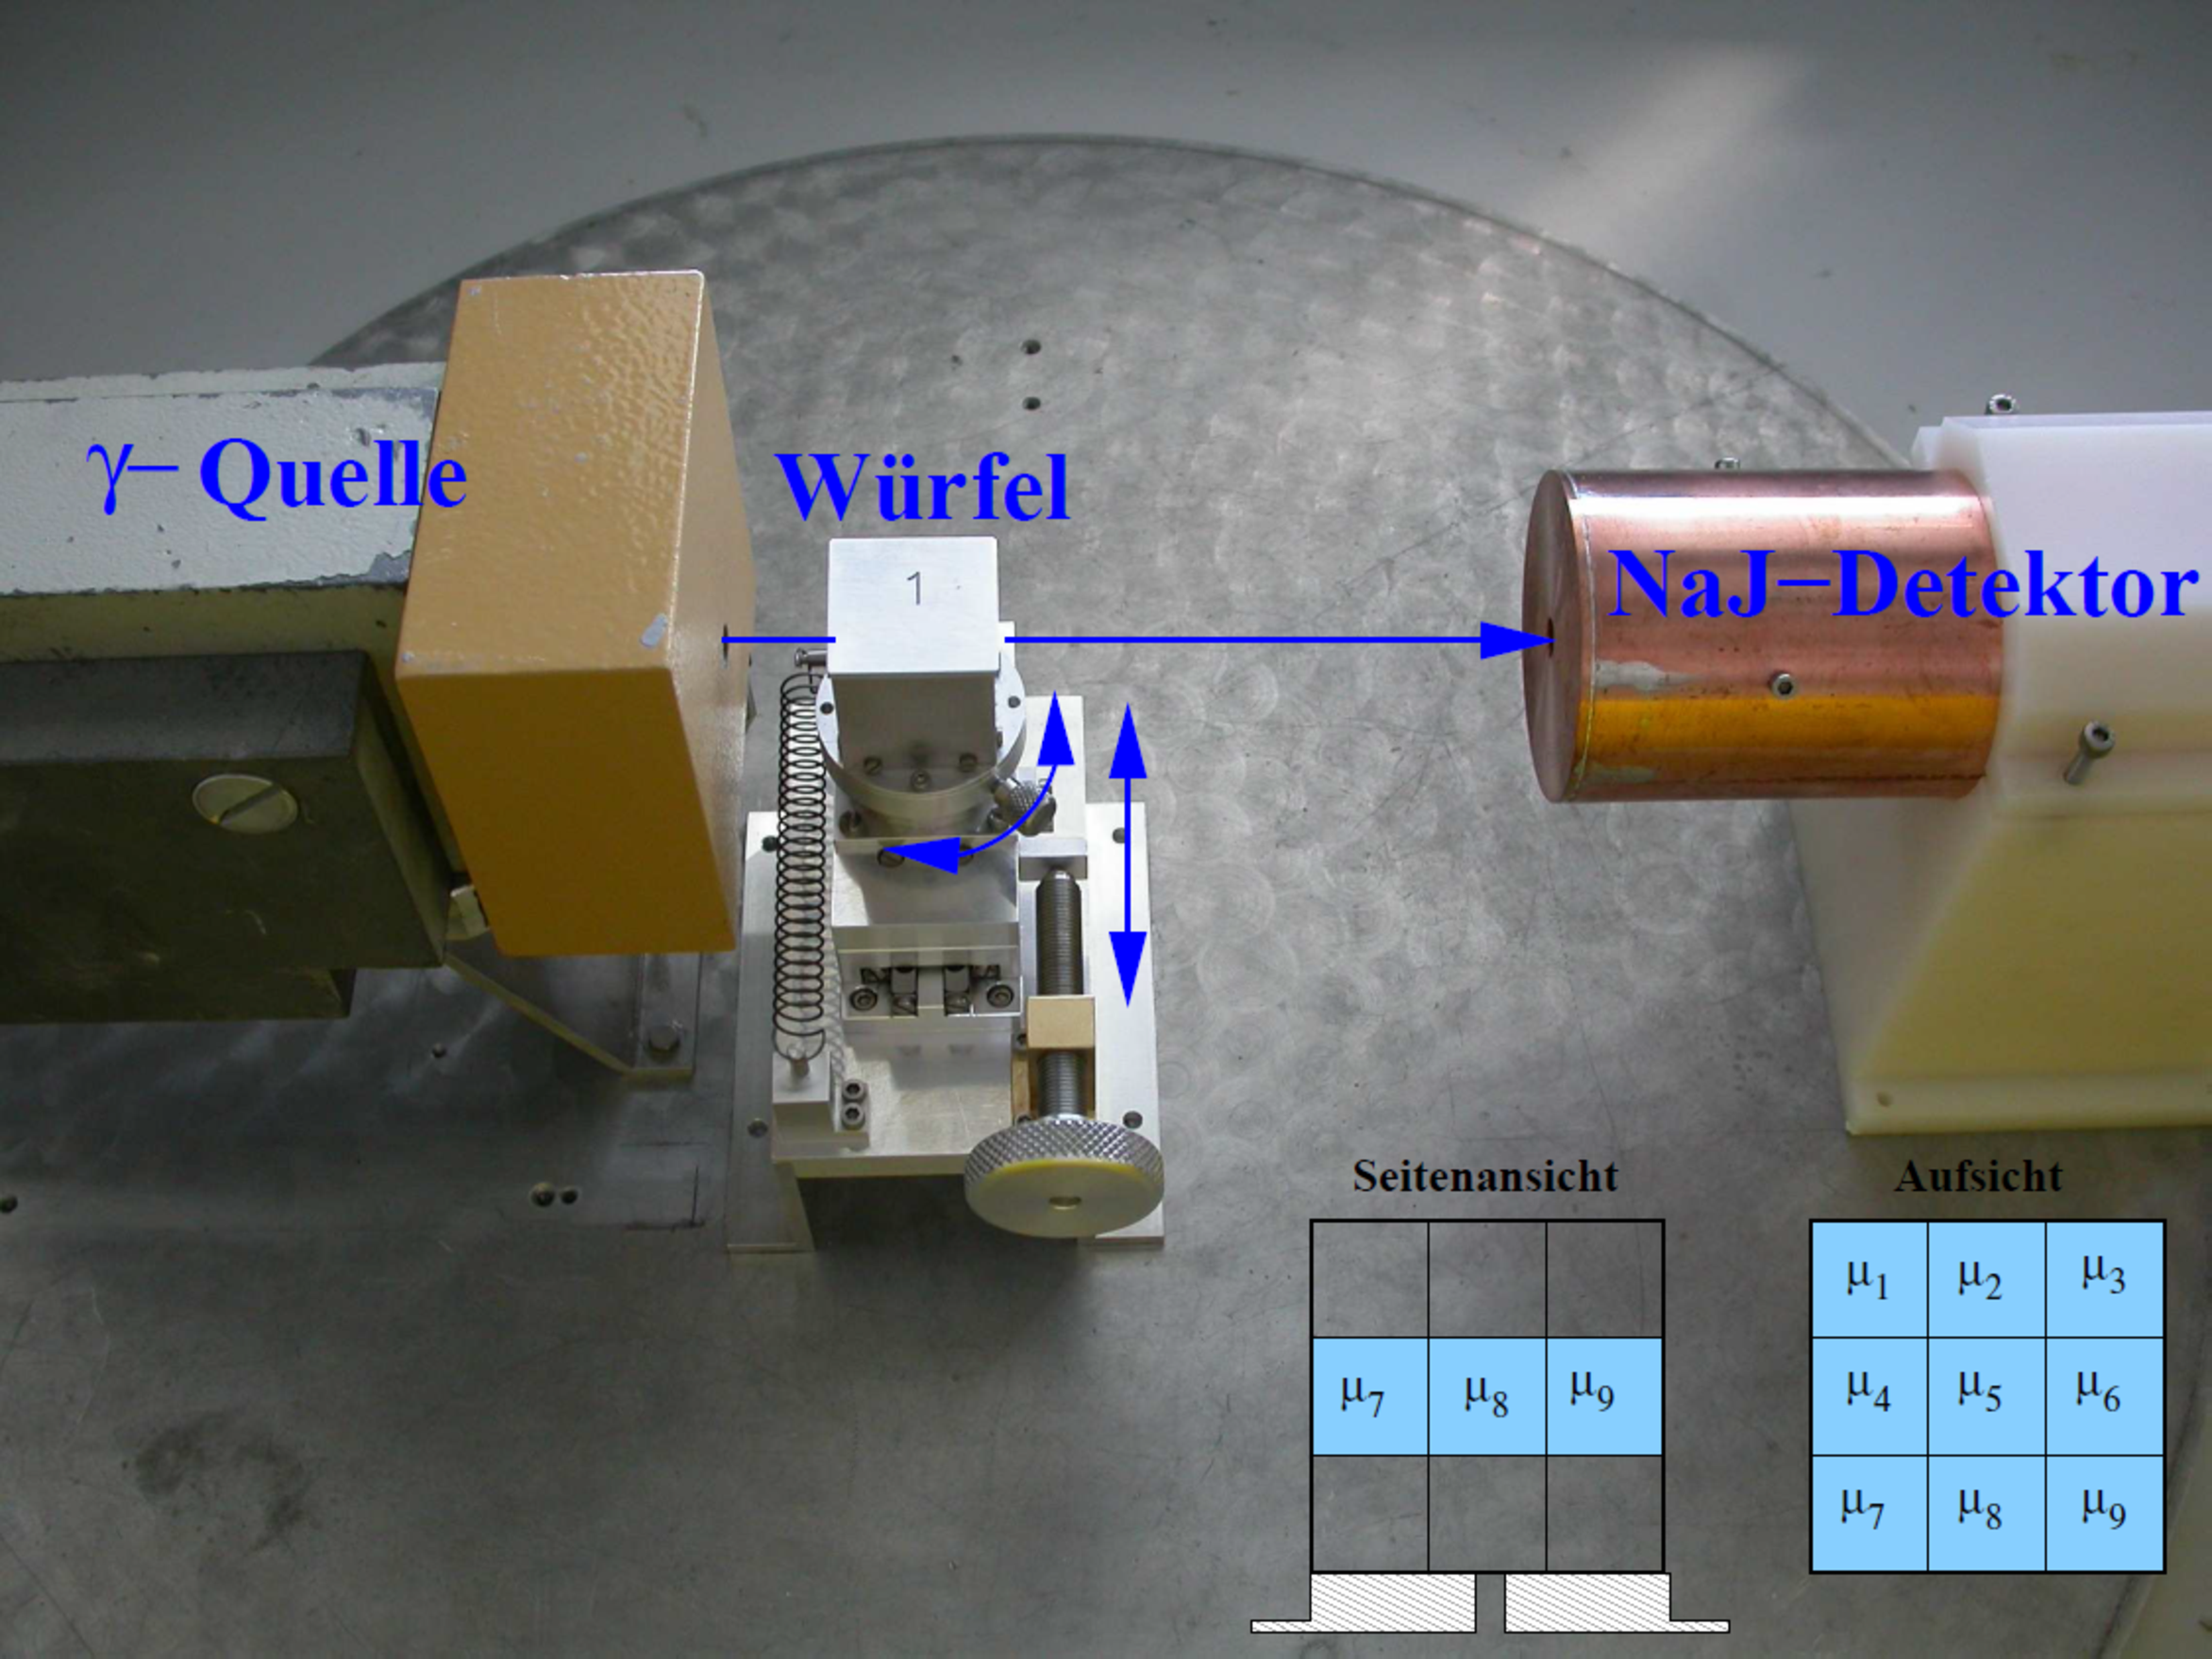
\includegraphics[width=0.6\textwidth]{pics/Aufbau.pdf}
  \caption{Bild des Versuchsaufbaus, außerdem ist die Zusammensetzung eines Würfels aus neun kleineren Würfeln zu erkennen \cite{anleitungb14}.}
  \label{fig: aufbau}
\end{figure}

Insgesamt werden in dem Versuch vier verschiedene Würfel untersucht. Eine Leermessung findet an
einem komplett leeren Würfel statt. Mit der Leermessung wird die Größe $I_0$ bestimmt \textbf{untersuchen}.
Außerdem soll so die Auswirkungen der Aluminiumhülle und der Umgebung gemessen werden.
Zum andern wird ein Würfel, der komplett aus Aluminium besteht und
ein aus Blei zusammengesetzter Würfel vermessen. Abschließend wird ein Würfel
unbekannter Zusammensetzung analysiert.

Die Analyse eines Würfels erfolgt in zwölf einzelne Messungen $i$,
bei jeder dieser Messungen wird die Ausrichtung des Würfels zum $\gamma$-Strahl geändert.
Eine Übersicht der verschiedenen Positionierungen befindest sich in der Abbildung \ref{fig: positionierung}.

\begin{figure}[h]
  \centering
  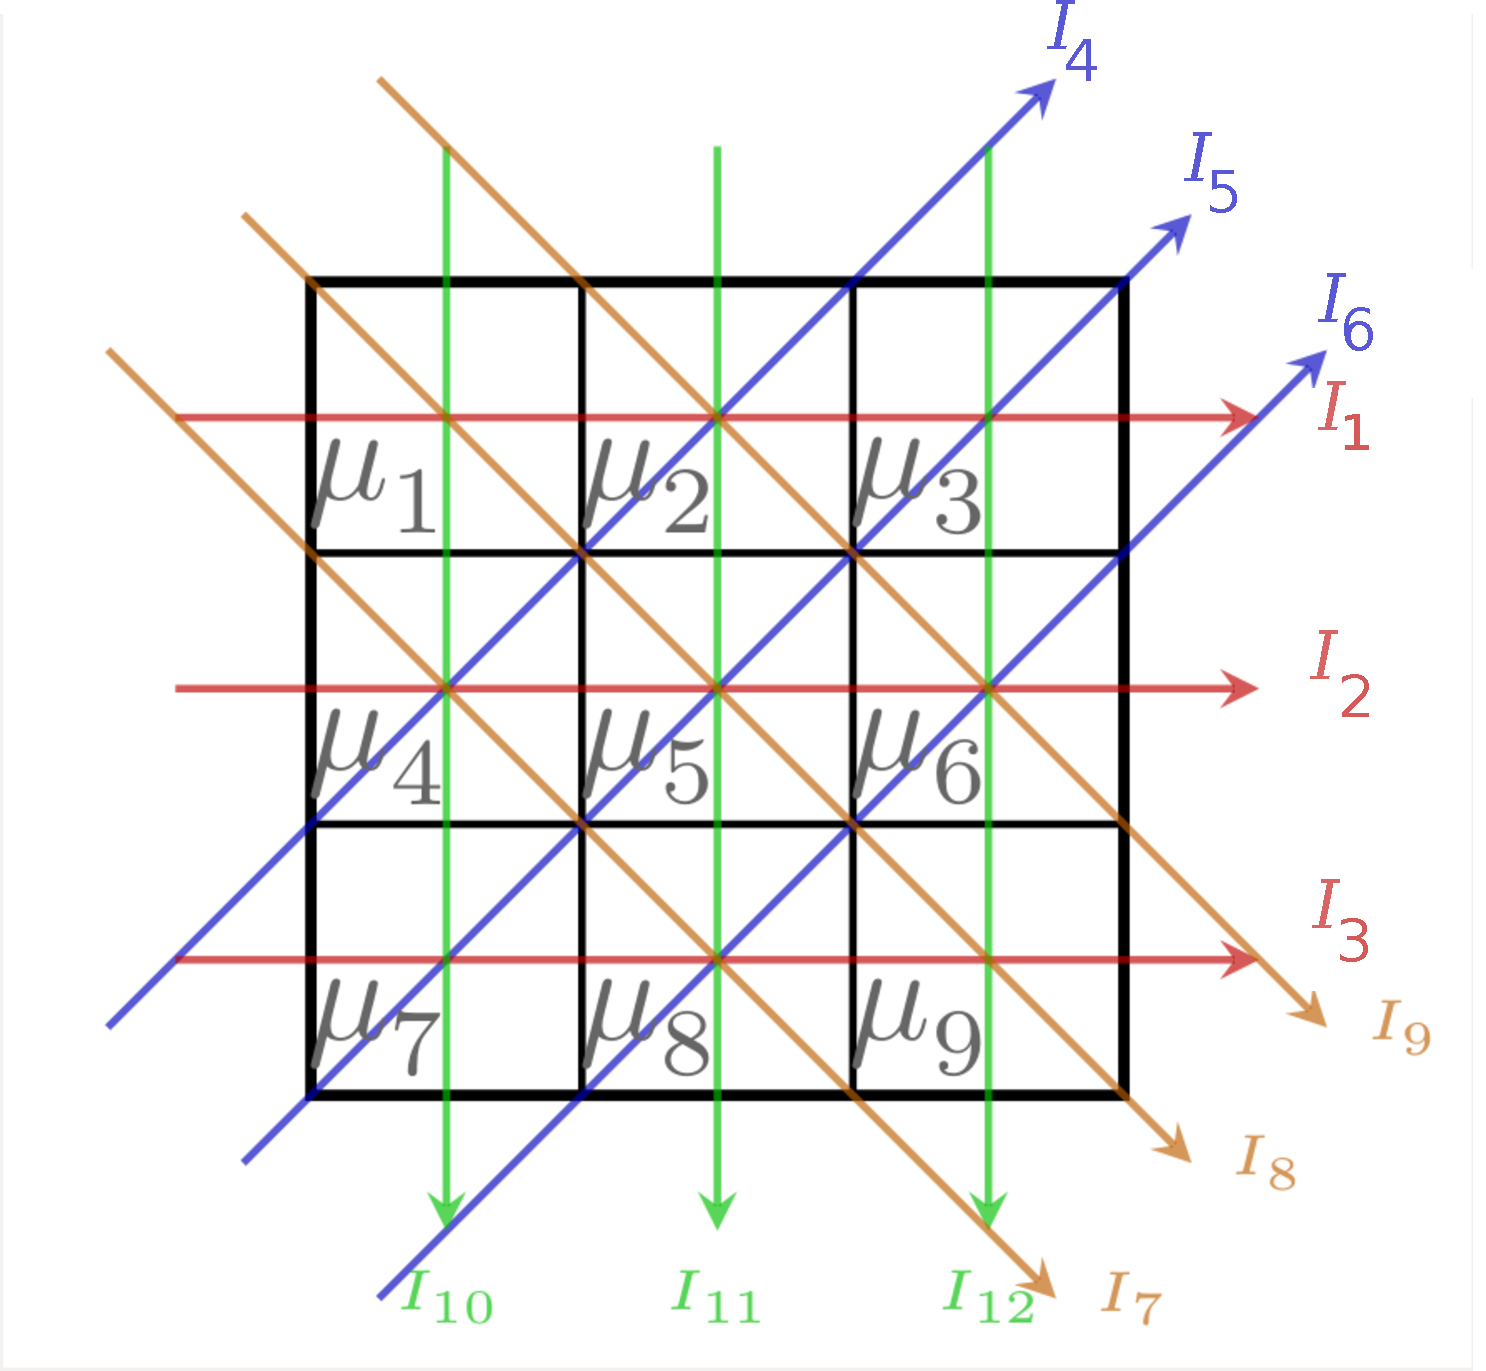
\includegraphics[width=0.6\textwidth]{pics/positionierung.pdf}
  \caption{Verschiedene Positionierunngen des Würfels. \cite{luckyjosh}.}
  \label{fig: positionierung}
\end{figure}

Insgesamt werden somit zwölf unterschiedliche Counts $N_i$ gemessen.
Eine Messung wird so lange durchgeführt bis der relative Fehler der poissonverteilten Counts
\begin{equation*}
  \sigma\ua{rel}=\frac{\sqrt{N}}{N}, \quad \text{Fehler\, Poisson}= \sqrt{N}
\end{equation*}
geringer als $3\%$ ist. Das entspricht einer Anzahl von etwa $N\approx 1200$.
Aus der Gleichung \eqref{eq: I_umge} wird ein Gleichungssystem, welches mit Hilfe einer
Matrixschreibweise geschrieben werden kann als

\begin{equation}
  \label{eq: matrix_absoprtionskoeffizienten}
  \underbrace{ l\begin{pmatrix} 1 & 1 & 1 & 0 & 0 & 0 & 0 & 0 & 0 \\ 0 & 0 & 0 & 1 & 1 & 1 & 0 & 0 & 0 \\ 0 & 0 & 0 & 0 & 0 & 0 & 1 & 1 & 1 \\ 0 & s & 0 & s & 0 & 0 & 0 & 0 & 0 \\ 0 & 0 & s & 0 & s & 0 & s & 0 & 0 \\ 0 & 0 & 0 & 0 & 0 & s & 0 & s & 0 \\ 0 & 0 & 0 & s & 0 & 0 & 0 & s & 0 \\ s & 0 & 0 & 0 & s & 0 & 0 & 0 & 0 \\ 0 & s & 0 & 0 & 0 & s & 0 & 0 & 0 \\ 1 & 0 & 0 & 1 & 0 & 0 & 1 & 0 & 0 \\ 0 & 1 & 0 & 0 & 1 & 0 & 0 & 1 & 0 \\ 0 & 0 & 1 & 0 & 0 & 1 & 0 & 0 & 1 \end{pmatrix} }_{=:\Phi}  \underbrace{ \begin{pmatrix}\mu_1 \\ \mu_2 \\ \mu_3 \\ \mu_4 \\ \mu_5 \\ \mu_6 \\ \mu_7 \\ \mu_8 \\ \mu_9 \end{pmatrix} }_{=:\vec{\mu}} = \underbrace{ \begin{pmatrix} I_1 \\ I_2 \\ I_3 \\ I_4 \\ I_5 \\ I_6 \\ I_7 \\ I_8 \\ I_9 \\ I_{10} \\ I_{11} \\ I_{12} \end{pmatrix} }_{ =:\vec{I}}, \quad s:=\sqrt{2}
\end{equation}
Das Lösungsverfahren für das Gleichungssystem wird in dem Kapitel \emph{Auswertung} näher beschrieben.

Die im Versuch verwendete $\gamma$-Strahlung wird mit Hilfe von $^{137}\ce{Cs}$ erzeugt (vgl. Abbildung \ref{fig: zerfall}).

\begin{figure}[h]
  \centering
  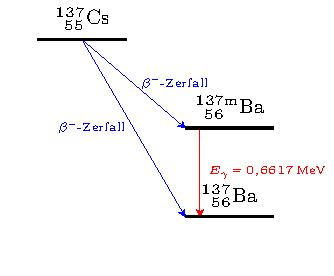
\includegraphics[width=0.5\textwidth]{pics/tikz-Energieschema.pdf}
  \caption{$^{137}\ce{Cs}$ als Quelle für $\gamma$-Strahlung im Versuch B14 \cite{luckyjosh}.}
  \label{fig: zerfall}
\end{figure}

Detektiert wird die abgeschwächte Strahlung mit Hilfe eines \emph{Szintillationsdetektors}.
Unter Einfluss von ionisierender Strahlung fängt dieser an zu leuchten bzw. emittiert Photonen $E\ua{photon}\propto E_\gamma$.
Die ausgesendeten Photonen werden mit einem \emph{Photomultiplier} erfasst. Wird ein Photon detektiert,
so gibt der Multiplier ein elektrisches Signal ab, wobei die Stärke des Signals proportional zur Energie des Photons ist.
Das vom \emph{Photomultiplier} ausgesendte Signal
wird an einen \emph{Diskriminator} weitergeleitet, der dieses je nach Signalstärke, einen Channel des
\emph{Multichannelanalyzer} zuweist. Der Multichannelanalyzer zählt, wie oft ein Signal einem Channel (insgesamt \textbf{1024}) zugewiesen wurde und
erstellt so ein Histogramm. Ist ein Channel auf HIGH gesetzt, werden alle anderen Channel so lang deaktiviert
bis der angeregte Channel wieder auf LOW fällt und somit sensitiv für ein neues Signal ist.

An einem beispielhaften Histogramm (vgl. Abb. \ref{fig: histo}) werden Wechselwirkungseffekte deutlich.
Hierbei ist die $x$-Achse ein Maß für die Energie der gemessenen Photonen.
Zu den Wechselwirkungseffekten gehören zum einen \emph{Compton Streuung}, \emph{Photoeffekt} und die \emph{Paarerzeugung}.
Jedoch tritt die Paarerzeug erst ab einer Energie von $E\ua{paar}\approx \SI{1}{\mega\eV}$ auf, die erzeugte $\gamma$-Strahlung
besitzt aber lediglich eine Energie von $E_{\gamma}\approx\SI{0.66}{\mega\eV}$ (vgl. Abb. \ref{fig: zerfall}).

Die Compton Streuung sorgt für eine Energieabschwächung der $\gamma$-Strahlung und ist deshalb für die Counts rechts von dem
orang eingefärbten Bereich. Die Verringerung der Counts im Breich von Channel 46, lässt sich mit dem Photoeffekt erklären.
In diesem Energiebereich liegt offensichtlich die Energie, um ein Elektron eines Bleiwürfels anzuregen.  % Stefan vlt schreibst du kurz in der Diskussion das die Abbildung auch nicht ideal ist und die einzelenen Effekt enicht wirklich erkennbar sind.

\begin{figure}[h]
  \centering
  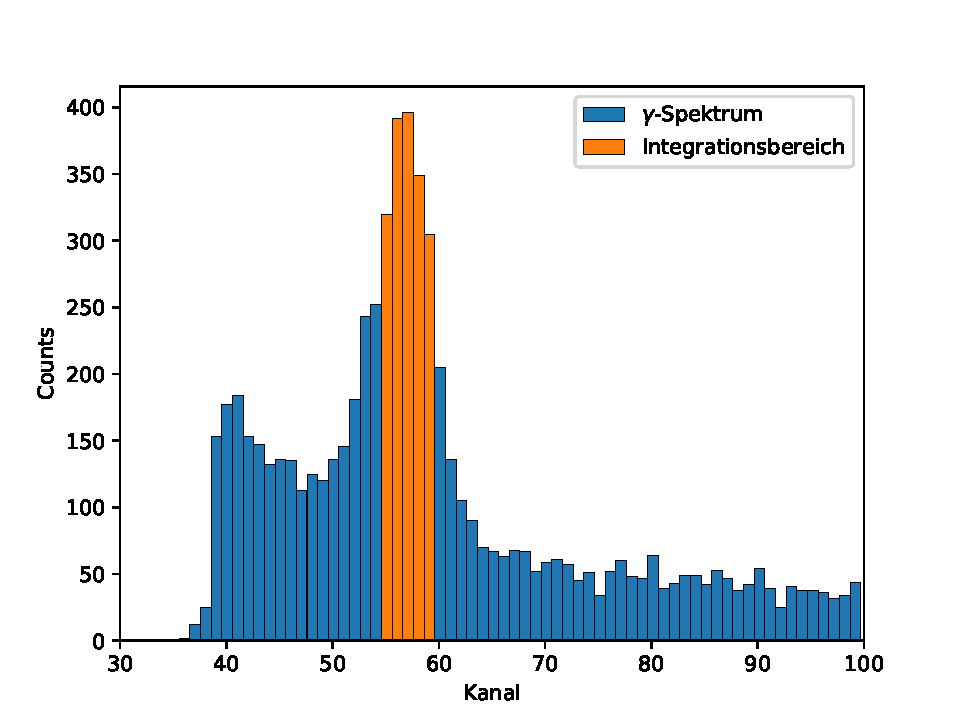
\includegraphics[width=0.6\textwidth]{hist/hist.pdf}
  \caption{Aufgenommenes Histogramm bei der Vermessung des Bleiwürfels in der Positionierung $I_5$.}
  \label{fig: histo}
\end{figure}
